%! TeX root = master.tex
% !TEX program = lualatex

\lecture{7}{2026-11-04}{Markov Chains}{}

\section{Towards reinforcement learning models}

This lecture marks a turning point of the course.
\begin{itemize}
    \item \textbf{So far: bandits.} Instantaneous reward after an action (the agent has immediate feedback); \textbf{memoryless environment} (the reward is only a function of the latest action, plus some noise); strong focus on ``squeezing out'' the lowest regret as a function of the system parameters.
    \item \textbf{Next: reinforcement learning (RL).} \textbf{Delayed reward} (the agent needs to craft \emph{sequences} of actions to do well); \textbf{environment with memory} (it remembers what happened in the past, so the current situation depends on previous actions); strong focus on algorithms that learn efficiently, less analysis of asymptotic behaviour.
    \item We therefore need \textbf{probabilistic models for memory}, with mathematical properties that allow us to reason about them, yet rich enough to model real systems. \textbf{Markov chains} are the most important such model, with many applications beyond RL. In RL, the environment will be a Markov chain whose transitions are influenced by the agent's actions (Markov decision processes, next lectures).
\end{itemize}
In this lecture:
\begin{itemize}
    \item we define (discrete-time, discrete-space) Markov chains, the transition matrix and the $n$-step transition probabilities (\textbf{Chapman-Kolmogorov} equations);
    \item we see that the evolution of a chain is entirely determined by its initial distribution $\boldsymbol{\mu}(0)$ and its transition matrix $P$;
    \item we \textbf{classify states}: transient / recurrent (null or positive), periodic / aperiodic, ergodic;
    \item we classify \textbf{chains}: communicating classes, closed and irreducible sets, and the \textbf{decomposition theorem};
    \item we study the long-term behaviour: the \textbf{ergodic theorem} and the \textbf{stationary distribution} $\pi$;
    \item we apply everything to \textbf{random walks} on $\mathbb{Z}$, $\mathbb{Z}^d$ and on general graphs.
\end{itemize}
\section{Definition and basic properties}

\subsection{The Markov condition}

Throughout, we study \textbf{discrete-time, discrete-space} Markov chains only:
\begin{itemize}
    \item discrete time: $t \in \mathbb{N}_0 = \{0, 1, 2, \dots\}$;
    \item discrete space: the \textbf{state space} $\mathcal{S}$ is a countable set (later, we will sometimes restrict $\mathcal{S}$ to be finite).
\end{itemize}

\begin{definition}[Markov chain]
The process $(X_0, X_1, X_2, \dots)$ with values in $\mathcal{S}$ is a \textbf{Markov chain} if it satisfies the \textbf{Markov condition}:
\[
\mathbb{P}\big[X_n = x \mid X_0 = x_0, X_1 = x_1, \dots, X_{n-1} = x_{n-1}\big] = \mathbb{P}\big[X_n = x \mid X_{n-1} = x_{n-1}\big]
\]
for all $n \geq 1$ and all $x, x_0, x_1, \dots, x_{n-1} \in \mathcal{S}$.
\end{definition}

Intuitively: \textbf{to predict the future, no knowledge of the past is useful beyond the current state}. Equivalently, conditionally on the present, the past and the future are independent. Markov chains are ``only one small step beyond independence'': an i.i.d.\ sequence is a (trivial) Markov chain where even the current state is useless to predict the future.

\subsection{Equivalent Markov conditions}

The Markov condition can be stated in several equivalent ways:
\begin{itemize}
    \item Conditioning on any finite set of past times, only the most recent one matters:
    \[
    \mathbb{P}\big[X_{n+1} = x \mid X_{n_1} = x_{n_1}, X_{n_2} = x_{n_2}, \dots, X_{n_k} = x_{n_k}\big] = \mathbb{P}\big[X_{n+1} = x \mid X_{n_k} = x_{n_k}\big]
    \]
    for all $n_1 < n_2 < \dots < n_k \leq n$.
    \item Predicting further in the future, only the current state matters:
    \[
    \mathbb{P}\big[X_{n+m} = x \mid X_0 = x_0, X_1 = x_1, \dots, X_n = x_n\big] = \mathbb{P}\big[X_{n+m} = x \mid X_n = x_n\big]
    \]
    for all $m, n \geq 0$.
\end{itemize}

\subsection{Homogeneous chains and the transition matrix}

\begin{definition}[Homogeneous chain]
The chain $X$ is \textbf{homogeneous} (time-shift-invariant) if
\[
\mathbb{P}\big[X_{n+1} = j \mid X_n = i\big] = \mathbb{P}\big[X_1 = j \mid X_0 = i\big] \quad \text{for all } n, i, j.
\]
\end{definition}

Homogeneity is the analogue of ``identically distributed'' for i.i.d.\ random variables: the transition mechanism does not change over time. \textbf{From now on, unless otherwise specified, we assume homogeneous chains.}

\begin{definition}[Transition matrix]
The \textbf{transition matrix} $P$ is the $|\mathcal{S}| \times |\mathcal{S}|$ matrix of transition probabilities
\[
p_{ij} = \mathbb{P}\big[X_{n+1} = j \mid X_n = i\big].
\]
Row $i$ is the distribution of the next state when the current state is $i$.
\end{definition}

$P$ is a \textbf{stochastic matrix}:
\begin{enumerate}
    \item[(a)] entries are non-negative: $p_{ij} \geq 0$;
    \item[(b)] row sums are equal to one: $\sum_j p_{ij} = 1$ (from state $i$, we must go somewhere).
\end{enumerate}
A Markov chain is conveniently drawn as a directed graph: one node per state, and an arrow $i \to j$ labelled $p_{ij}$ whenever $p_{ij} > 0$.

\subsection{$n$-step transition matrix}

\begin{definition}[$n$-step transition probabilities]
\[
P_n : \quad p_{ij}(n) = \mathbb{P}\big[X_{m+n} = j \mid X_m = i\big] \qquad (\text{independent of } m \text{ by homogeneity}),
\]
with $P_1 = P$ and $P_0 = I$, i.e.\ $p_{ij}(0) = \delta_{ij}$.
\end{definition}

\begin{remark}[Example: a two-state chain]
Let $\mathcal{S} = \{1, 2\}$ with
\[
P_1 = P = \begin{pmatrix} 1/2 & 1/2 \\ 3/4 & 1/4 \end{pmatrix},
\quad
P_2 = \begin{pmatrix} 0.625 & 0.375 \\ 0.563 & 0.438 \end{pmatrix},
\quad
P_3 = \begin{pmatrix} 0.594 & 0.406 \\ 0.609 & 0.391 \end{pmatrix},
\quad
P_{10} = \begin{pmatrix} 0.600 & 0.400 \\ 0.600 & 0.400 \end{pmatrix}.
\]
After $10$ steps, we end up in state $1$ or $2$ with pretty much the same probability \textbf{regardless of where we started}: both rows of $P_{10}$ are (almost) identical. The chain ``forgets'' its initial state. This is \textbf{ergodicity}, to which we return at the end of the lecture.
\end{remark}

\begin{center}
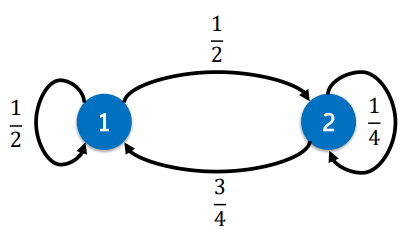
\includegraphics[width=0.4\linewidth]{images/img_20261106_145715.png}
\end{center}

\subsection{Chapman-Kolmogorov equations}

\begin{theorem}[Chapman-Kolmogorov]
For all $m, n \geq 0$ and all $i, j \in \mathcal{S}$:
\[
p_{ij}(m+n) = \sum_{k} p_{ik}(m)\, p_{kj}(n).
\]
In matrix form: $P_{m+n} = P_m P_n$. Hence $P_n = P^n$: the $n$-step transition matrix is the $n$-th power of the transition matrix.
\end{theorem}

\begin{proof}
To go from $i$ to $j$ in $m+n$ steps, we must be in some state $k$ at time $m$:
\begin{align*}
p_{ij}(m+n) &= \mathbb{P}\big[X_{m+n} = j \mid X_0 = i\big] \\
&= \sum_k \mathbb{P}\big[X_{m+n} = j, X_m = k \mid X_0 = i\big] && \text{(law of total probability)} \\
&= \sum_k \mathbb{P}\big[X_{m+n} = j \mid X_m = k, X_0 = i\big]\,\mathbb{P}\big[X_m = k \mid X_0 = i\big] && \big(\mathbb{P}[A, B \mid C] = \mathbb{P}[A \mid B, C]\,\mathbb{P}[B \mid C]\big) \\
&= \sum_k \mathbb{P}\big[X_{m+n} = j \mid X_m = k\big]\,\mathbb{P}\big[X_m = k \mid X_0 = i\big] && \text{(Markov property)} \\
&= \sum_k p_{kj}(n)\, p_{ik}(m).
\end{align*}
By induction, $P_n = P_{n-1}P_1 = \dots = P^n$.
\end{proof}

\subsection{Evolution of the marginal distribution of $X_n$}

\begin{definition}[Marginal distribution]
$\mu_i(n) = \mathbb{P}[X_n = i]$, and $\boldsymbol{\mu}(n) = [\mu_1(n), \mu_2(n), \dots]$ is the distribution of $X_n$, written as a \textbf{row vector}.
\end{definition}

\begin{theorem}[Lemma]
$\boldsymbol{\mu}(m+n) = \boldsymbol{\mu}(m) P^n$. In particular, $\boldsymbol{\mu}(n) = \boldsymbol{\mu}(0) P^n$.
\end{theorem}

\begin{proof}
By the law of total probability,
\[
\mu_j(m+n) = \mathbb{P}\big[X_{m+n} = j\big] = \sum_i \mathbb{P}\big[X_{m+n} = j \mid X_m = i\big]\,\mathbb{P}\big[X_m = i\big] = \sum_i \mu_i(m)\, p_{ij}(n) = \big(\boldsymbol{\mu}(m) P_n\big)_j,
\]
and $P_n = P^n$ by Chapman-Kolmogorov.
\end{proof}

\textbf{Key point}: the random evolution of a Markov chain is entirely determined by
\begin{itemize}
    \item $\boldsymbol{\mu}(0)$: the \textbf{initial conditions};
    \item $P$: the \textbf{dynamics}.
\end{itemize}
In fact, the whole joint law is determined: $\mathbb{P}[X_0 = x_0, X_1 = x_1, \dots, X_n = x_n] = \mu_{x_0}(0)\, p_{x_0x_1} p_{x_1x_2}\cdots p_{x_{n-1}x_n}$ (chain rule $+$ Markov property).

\subsection{Example: the simple random walk}

\begin{definition}[Simple random walk on $\mathbb{Z}$]
$\mathcal{S} = \{0, \pm1, \pm2, \pm3, \dots\} = \mathbb{Z}$, and
\[
p_{ij} = \begin{cases} p & j = i+1, \\ q = 1-p & j = i-1, \\ 0 & \text{otherwise.} \end{cases}
\]
At each step, we move one unit to the right with probability $p$ and one unit to the left with probability $q$.
\end{definition}

\textbf{$n$-step transition probabilities.} To go from $i$ to $j$ in $n$ steps, we need to make $j - i$ more steps to the right than to the left. With $r$ right steps and $l$ left steps:
\[
r + l = n, \qquad r - l = j - i \quad\Rightarrow\quad r = \tfrac12(n + j - i),
\]
which must be an integer. There are $\binom{n}{r}$ sequences of length $n$ with $r$ right steps and $l = n - r$ left steps, each with probability $p^r q^l$. Hence
\[
p_{ij}(n) = \begin{cases} \displaystyle\binom{n}{\frac12(n+j-i)}\, p^{\frac12(n+j-i)}\, q^{\frac12(n-j+i)} & n + j - i \text{ even}, \\[2ex] 0 & \text{otherwise.} \end{cases}
\]
Starting from $0$, the distribution $\boldsymbol{\mu}(n)$ spreads out over time (and drifts to the right if $p > q$); note the parity constraint: at even times, the walk is at an even position.

\begin{center}
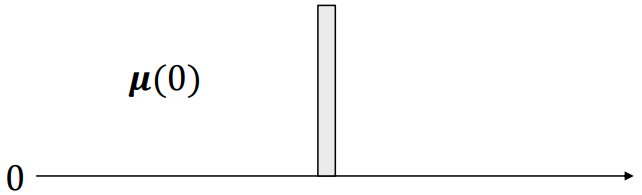
\includegraphics[width=0.3\linewidth]{images/img_20261106_152652.png}
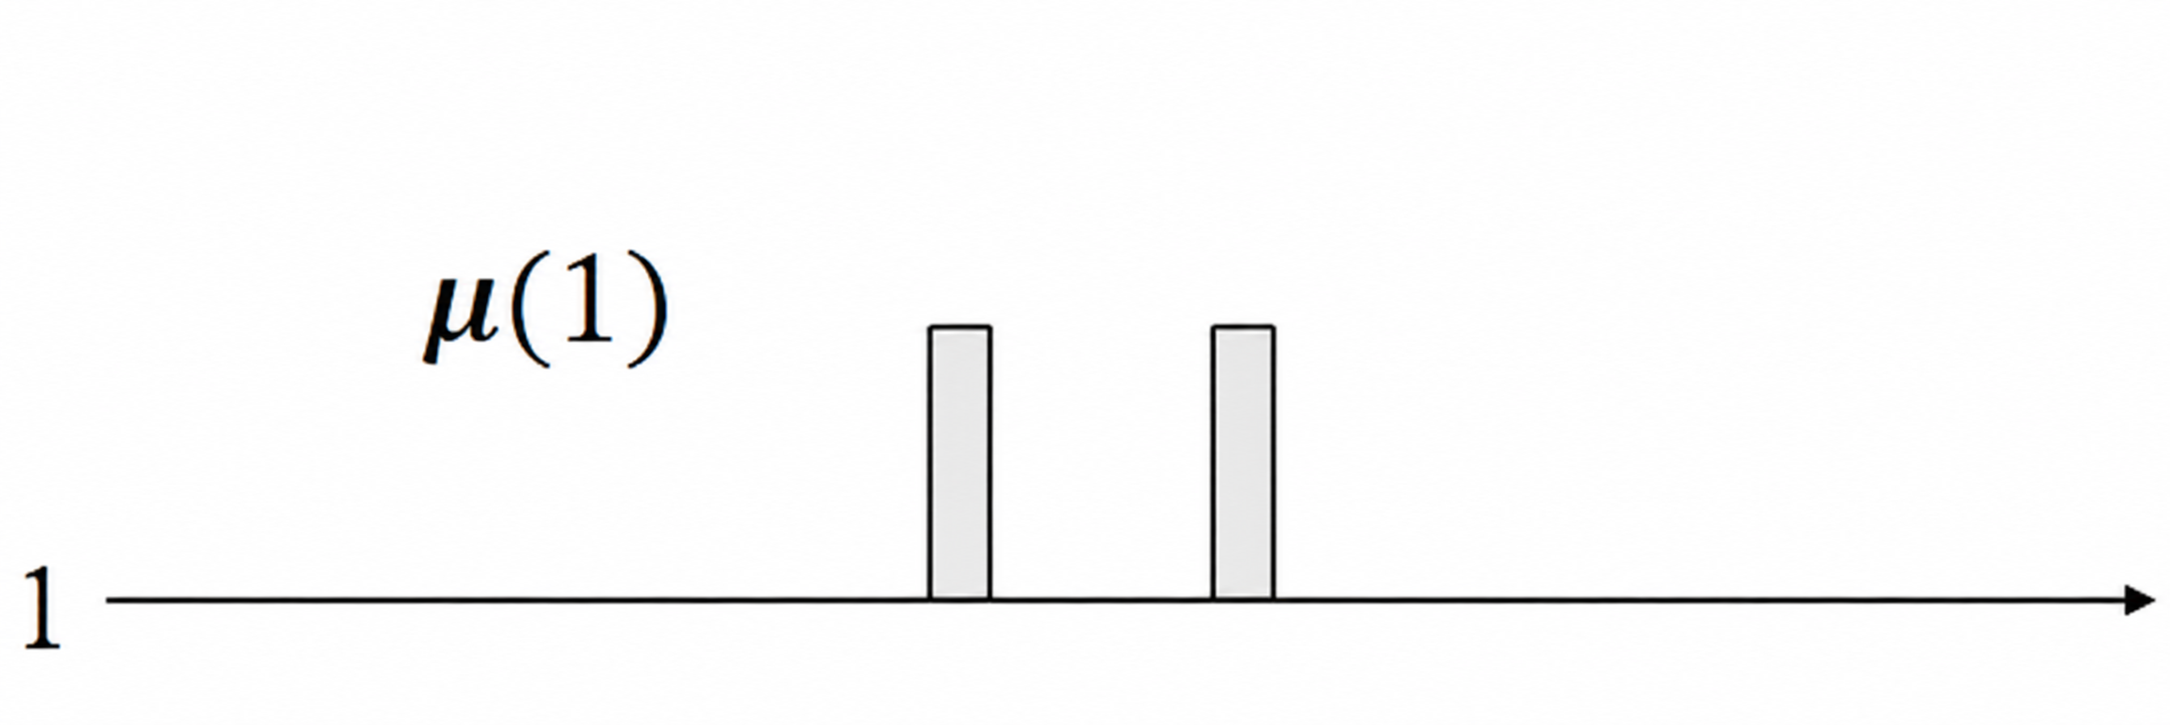
\includegraphics[width=0.3\linewidth]{images/img_20261106_152730.png}
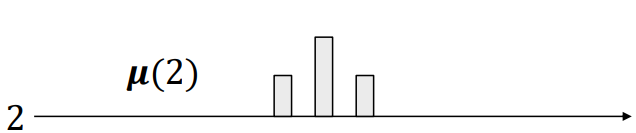
\includegraphics[width=0.3\linewidth]{images/img_20261106_152745.png}
\end{center}

\subsection{Chapman-Kolmogorov $\not\Rightarrow$ Markov}

Chapman-Kolmogorov is a \textbf{necessary but not sufficient} condition for being a Markov chain. Counterexample:
\begin{itemize}
    \item Let $Y_1, Y_3, Y_5, \dots$ be an i.i.d.\ sequence of random variables with values $\pm1$, each with probability $1/2$: $\mathbb{P}[Y_{2k+1} = -1] = \mathbb{P}[Y_{2k+1} = +1] = 1/2$.
    \item Define the even terms as products of their neighbours: $Y_{2k} = Y_{2k-1}\,Y_{2k+1}$.
    \item The sequence $Y_2, Y_4, Y_6, \dots$ is also i.i.d.\ with the same distribution, and adjacent pairs $Y_{2k}$, $Y_{2k+1}$ are also independent (knowing $Y_{2k+1}$, the product $Y_{2k-1}Y_{2k+1}$ is still a fair $\pm1$). Therefore the whole sequence is \textbf{pairwise independent}.
    \item Hence, for all $n \geq 1$, $p_{ij}(n) = \mathbb{P}[Y_{m+n} = j \mid Y_m = i] = \frac12$: all $n$-step matrices equal the matrix with all entries $\frac12$, which trivially satisfies $P_{m+n} = P_mP_n$. Chapman-Kolmogorov holds.
    \item But $Y$ is \textbf{not} a Markov chain:
    \[
    \mathbb{P}\big[Y_{2k+1} = 1 \mid Y_{2k} = -1\big] = \tfrac12, \qquad \text{but} \qquad \mathbb{P}\big[Y_{2k+1} = 1 \mid Y_{2k} = -1, Y_{2k-1} = 1\big] = 0,
    \]
    since $Y_{2k+1} = Y_{2k}/Y_{2k-1} = -1$. Knowing one more past value changes the prediction.
\end{itemize}

\section{Classification of states}

\subsection{Recurrence and transience}

\begin{definition}[Recurrent and transient states]
State $i$ is \textbf{recurrent} (or \emph{persistent}) if
\[
\mathbb{P}\big[X_n = i \text{ for some } n \geq 1 \mid X_0 = i\big] = 1,
\]
i.e.\ starting from $i$, the chain returns to $i$ with certainty. State $i$ is \textbf{transient} otherwise, i.e.\ if
\[
\mathbb{P}\big[X_n = i \text{ for some } n \geq 1 \mid X_0 = i\big] < 1.
\]
\end{definition}

\begin{remark}
Starting at $i$ is important in the definition: we may never visit state $i$ starting from some $j \neq i$, even though $i$ is recurrent!

By the Markov property, each return to $i$ ``restarts'' the chain. Hence a recurrent state is visited \textbf{infinitely often} (with probability $1$), whereas a transient state is visited only a finite number of times (a geometric number of returns, with success probability $1 - f_{ii}$ below): it is eventually abandoned.
\end{remark}

\begin{definition}[First passage probabilities]
The probability of a \textbf{first visit} to state $j$, starting at state $i$, in exactly $n$ steps:
\[
f_{ij}(n) = \mathbb{P}\big[X_1 \neq j, X_2 \neq j, \dots, X_{n-1} \neq j, X_n = j \mid X_0 = i\big], \qquad f_{ij}(0) = 0.
\]
The probability of \textbf{ever} visiting $j$ after $i$:
\[
f_{ij} = \sum_{n=1}^\infty f_{ij}(n).
\]
\end{definition}

The events $\{$first visit at time $n\}$ are disjoint, which is why we can sum them. Note:
\[
j \text{ is recurrent} \iff f_{jj} = 1.
\]

\subsection{Linking transition probabilities and first passage times}

We now relate $p_{ij}(n)$ (easy to compute: powers of $P$) to $f_{ij}(n)$ (which defines recurrence). The tool is \textbf{probability generating functions}.

\begin{definition}[Generating functions]
For $|s| < 1$:
\[
P_{ij}(s) = \sum_{n=0}^\infty s^n p_{ij}(n) \quad (p_{ij}(0) = \delta_{ij}), \qquad F_{ij}(s) = \sum_{n=0}^\infty s^n f_{ij}(n) \quad (f_{ij}(0) = 0).
\]
\end{definition}

\begin{theorem}
\begin{enumerate}
    \item[(a)] $P_{ii}(s) = 1 + F_{ii}(s)\,P_{ii}(s)$;
    \item[(b)] $P_{ij}(s) = F_{ij}(s)\,P_{jj}(s)$ for $i \neq j$.
\end{enumerate}
In one formula: $P_{ij}(s) = F_{ij}(s)\,P_{jj}(s) + \delta_{ij}$ for any $i, j$.
\end{theorem}

\begin{proof}
Fix two states $i, j$, and define for $m \geq 1$ the events
\[
A_m = \{X_m = j\}, \qquad B_m = \{X_k \neq j \text{ for } 1 \leq k < m,\ X_m = j\} \quad \text{(first visit to $j$ happens at time $m$)}.
\]
The $B_m$ are disjoint, and $B_m \Rightarrow A_m$. If $A_m$ occurs, the first visit to $j$ happened at some time $r \in \{1, \dots, m\}$, so
\[
p_{ij}(m) = \mathbb{P}\big[A_m \mid X_0 = i\big] = \sum_{r=1}^m \mathbb{P}\big[A_m, B_r \mid X_0 = i\big].
\]
Moreover,
\[
\mathbb{P}\big[A_m, B_r \mid X_0 = i\big] = \mathbb{P}\big[A_m \mid B_r, X_0 = i\big]\,\mathbb{P}\big[B_r \mid X_0 = i\big] = \underbrace{\mathbb{P}\big[A_m \mid X_r = j\big]}_{p_{jj}(m-r)}\,\underbrace{\mathbb{P}\big[B_r \mid X_0 = i\big]}_{f_{ij}(r)},
\]
where $\mathbb{P}[A_m \mid B_r, X_0 = i] = \mathbb{P}[A_m \mid X_r = j]$ follows from the Markov property: $A_m$ depends only on $X_r = j$, not on what happened before. Hence
\[
p_{ij}(m) = \sum_{r=1}^m f_{ij}(r)\, p_{jj}(m - r) \qquad (m = 1, 2, \dots).
\]
This is a \textbf{convolution}, which becomes a \textbf{multiplication in the transform domain}:
\begin{align*}
P_{ij}(s) &= \sum_{m=1}^\infty s^m p_{ij}(m) + \delta_{ij}
= \sum_{m=1}^\infty s^m \sum_{r=1}^m f_{ij}(r)\, p_{jj}(m-r) + \delta_{ij} \\
&= \sum_{m=1}^\infty \sum_{r=1}^m s^r f_{ij}(r)\; s^{m-r} p_{jj}(m-r) + \delta_{ij}
= \sum_{r=1}^\infty s^r f_{ij}(r) \sum_{m=r}^\infty s^{m-r} p_{jj}(m-r) + \delta_{ij} \\
&= F_{ij}(s)\, P_{jj}(s) + \delta_{ij},
\end{align*}
where we exchanged the two sums (all terms are non-negative).
\end{proof}

\subsection{Recurrence/transience in terms of $n$-step transition probabilities}

\begin{theorem}
\begin{itemize}
    \item $\sum_n p_{jj}(n) = \infty \iff j$ is recurrent; in that case $\sum_n p_{ij}(n) = \infty$ for all $i$ such that $f_{ij} > 0$.
    \item $\sum_n p_{jj}(n) < \infty \iff j$ is transient; in that case $\sum_n p_{ij}(n) < \infty$ for all $i$.
\end{itemize}
\end{theorem}

In words: the infinite series of $n$-step \emph{return} probabilities is infinite/finite exactly when the series of $n$-step transition probabilities from any other state (that can reach $j$) is infinite/finite. This is the practical criterion: recurrence is defined through $f_{jj}$, but checked through $p_{jj}(n)$, which can be computed.

\begin{remark}[Interpretation]
$\sum_{n\geq1} p_{jj}(n) = \sum_{n \geq 1}\mathbb{E}\big[\mathbf{1}\{X_n = j\} \mid X_0 = j\big] = \mathbb{E}[\text{number of returns to } j \mid X_0 = j]$. So the theorem says: $j$ is recurrent iff the expected number of returns is infinite, consistent with ``a recurrent state is visited infinitely often''.
\end{remark}

\subsection{Classification as a function of the recurrence time}

\begin{definition}[First visit time]
\[
T_j = \min\{n \geq 1 : X_n = j\}, \qquad T_j = \infty \text{ if the chain never visits } j.
\]
\end{definition}

Note: $\mathbb{P}[T_i = \infty \mid X_0 = i] > 0$ iff $i$ is transient, in which case $\mathbb{E}[T_i \mid X_0 = i] = \infty$.

\begin{definition}[Mean recurrence time]
\[
\mu_i = \mathbb{E}\big[T_i \mid X_0 = i\big] = \begin{cases} \sum_n n f_{ii}(n) & \text{if } i \text{ is recurrent}, \\ \infty & \text{if } i \text{ is transient.} \end{cases}
\]
\end{definition}

(Careful: the mean recurrence time $\mu_i$ is a number; do not confuse it with the marginal distribution $\mu_i(n)$.)

\begin{definition}[Null and positive recurrence]
A recurrent state $i$ is called
\begin{itemize}
    \item \textbf{null-recurrent} if $\mu_i = \infty$;
    \item \textbf{positive-recurrent} if $\mu_i < \infty$.
\end{itemize}
\end{definition}

A null-recurrent state is ``on the edge'': we are sure to come back, but the expected time to come back is infinite.

\begin{theorem}
A recurrent state $i$ is null $\iff$ $p_{ii}(n) \to 0$ as $n \to \infty$.
\end{theorem}

\subsection{Periodicity}

\begin{definition}[Period]
The \textbf{period} $d_i$ of state $i$ is
\[
d_i = \gcd\{n \geq 1 : p_{ii}(n) > 0\}.
\]
State $i$ is \textbf{periodic} if $d_i > 1$, and \textbf{aperiodic} otherwise ($d_i = 1$).
\end{definition}

In words: returns to $i$ are only possible at times that are multiples of $d_i$. Note that $p_{ii}(d_i)$ itself need not be positive: what matters is the $\gcd$ of all possible return times. A self-loop ($p_{ii} > 0$) immediately makes $i$ aperiodic.

\begin{definition}[Ergodic state]
A state $i$ is \textbf{ergodic} if it is positive-recurrent and aperiodic.
\end{definition}

\begin{center}
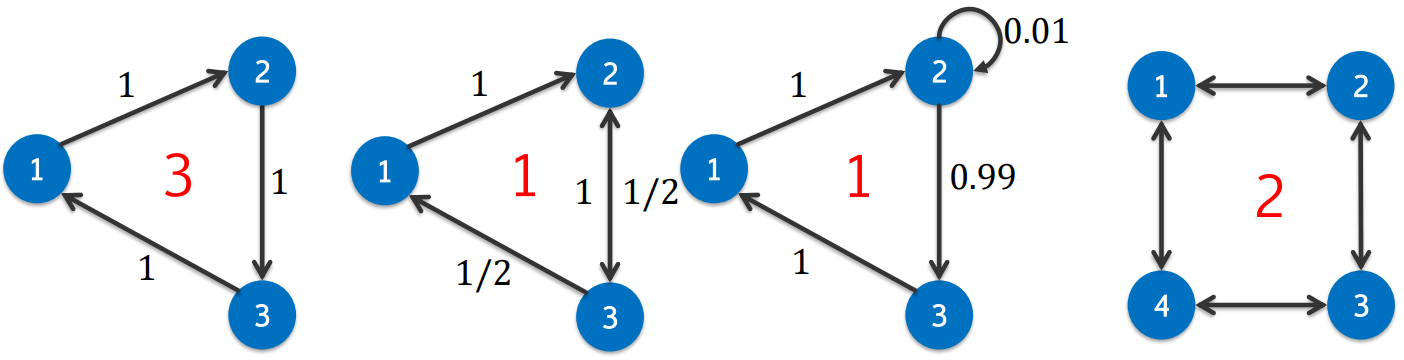
\includegraphics[width=\linewidth]{images/img_20261106_161012.png}
\end{center}

\textbf{Examples} (slide 18, from left to right):
\begin{enumerate}
    \item Deterministic cycle $1 \to 2 \to 3 \to 1$: returns to $1$ only at times $3, 6, 9, \dots$ $\Rightarrow$ period $3$.
    \item $1 \to 2 \to 3$ with probability $1$, then from $3$ back to $1$ or to $2$ with probability $1/2$ each: return times to $1$ include $3$ ($1\to2\to3\to1$) and $5$ ($1\to2\to3\to2\to3\to1$), and $\gcd(3,5) = 1$ $\Rightarrow$ aperiodic.
    \item Cycle $1 \to 2 \to 3 \to 1$ with a self-loop of probability $0.01$ at state $2$: return times $3$ and $4$, $\gcd(3,4) = 1$ $\Rightarrow$ aperiodic. Even a tiny self-loop destroys periodicity (the exact value of the probability does not matter).
    \item Square $1 \leftrightarrow 2 \leftrightarrow 3 \leftrightarrow 4 \leftrightarrow 1$ (bidirectional edges): every return takes an even number of steps $\Rightarrow$ period $2$.
\end{enumerate}

\section{Classification of chains}

\subsection{Communicating states}

We now look at the relationships of states to each other.

\begin{definition}[Communication]
\begin{itemize}
    \item $i$ \textbf{communicates with} $j$ (written $i \to j$) if $p_{ij}(m) > 0$ for some $m \geq 0$ ($j$ is reachable from $i$).
    \item $i$ \textbf{intercommunicates with} $j$ (written $i \leftrightarrow j$) if $i \to j$ and $j \to i$.
\end{itemize}
\end{definition}

Properties:
\begin{enumerate}
    \item[(a)] For $i \neq j$: $i \to j \iff f_{ij} > 0$.
    \item[(b)] For $i = j$: $i \to i$ always, because $p_{ii}(0) = 1$.
    \item[(c)] $i \leftrightarrow j$ and $j \leftrightarrow k$ $\Rightarrow$ $i \leftrightarrow k$ (by Chapman-Kolmogorov, $p_{ik}(m+n) \geq p_{ij}(m)p_{jk}(n) > 0$).
\end{enumerate}
Hence ``$\leftrightarrow$'' is reflexive, symmetric and transitive: it is an \textbf{equivalence relation}, which \textbf{partitions $\mathcal{S}$ into equivalence classes} of states (the communicating classes, i.e.\ the strongly connected components of the transition graph).

\subsection{Properties of classes of states}

\begin{theorem}
If $i \leftrightarrow j$, then:
\begin{enumerate}
    \item[(a)] $i$ and $j$ have the same period;
    \item[(b)] $i$ is transient $\iff$ $j$ is transient;
    \item[(c)] $i$ is null-recurrent $\iff$ $j$ is null-recurrent;
    \item[(d)] $i$ is positive-recurrent $\iff$ $j$ is positive-recurrent.
\end{enumerate}
In other words, periodicity, transience, null-recurrence and positive recurrence are \textbf{class properties}.
\end{theorem}

\begin{proof}[Proof of (b)]
If $i \leftrightarrow j$, there exist $m, n \geq 0$ such that
\[
\alpha = p_{ij}(m)\, p_{ji}(n) > 0.
\]
By Chapman-Kolmogorov (keeping only one term of the sum: go from $i$ to $j$ in $m$ steps, loop from $j$ to $j$ in $r$ steps, come back to $i$ in $n$ steps),
\[
p_{ii}(m + r + n) \geq p_{ij}(m)\, p_{jj}(r)\, p_{ji}(n) = \alpha\, p_{jj}(r) \qquad \text{for any } r \geq 0.
\]
Summing over $r$:
\[
\sum_r p_{ii}(r) < \infty \;\Rightarrow\; \sum_r p_{jj}(r) \leq \frac{1}{\alpha}\sum_r p_{ii}(m+r+n) < \infty.
\]
In other words, $i$ transient implies $j$ transient. By symmetry, $j$ transient implies $i$ transient.
\end{proof}

\subsection{Closed and irreducible sets of states}

\begin{definition}[Closed and irreducible sets]
A set $C \subset \mathcal{S}$ of states is called
\begin{enumerate}
    \item[(a)] \textbf{closed} (or \textbf{absorbing}) if $p_{ij} = 0$ for all $i \in C$, $j \notin C$: ``we can never leave'';
    \item[(b)] \textbf{irreducible} if $i \leftrightarrow j$ for all $i, j \in C$: ``we can move freely inside $C$''.
\end{enumerate}
\end{definition}

Because of the preceding theorem, all states in an irreducible set share the same properties (periodic/aperiodic, and transient/null-recurrent/positive-recurrent). If the whole $\mathcal{S}$ is irreducible, we say that the \textbf{chain} has these shared properties (e.g.\ ``an irreducible, aperiodic, positive-recurrent chain'').

\begin{remark}[How to classify states in practice]
Arrows represent any positive probability: the exact values do not matter to classify states (except to distinguish null from positive recurrence in infinite chains, and recurrence from transience in infinite chains).
\begin{enumerate}
    \item Draw the transition graph and find the communicating classes (groups of states that can reach each other).
    \item A class from which an arrow leaves is \textbf{not closed}; in a finite chain, it is \textbf{transient}. A closed finite class is positive-recurrent.
    \item For each class, compute the period: $\gcd$ of the lengths of the cycles through one of its states (a self-loop $\Rightarrow$ aperiodic).
\end{enumerate}
\end{remark}

\subsection{Examples}

\begin{center}
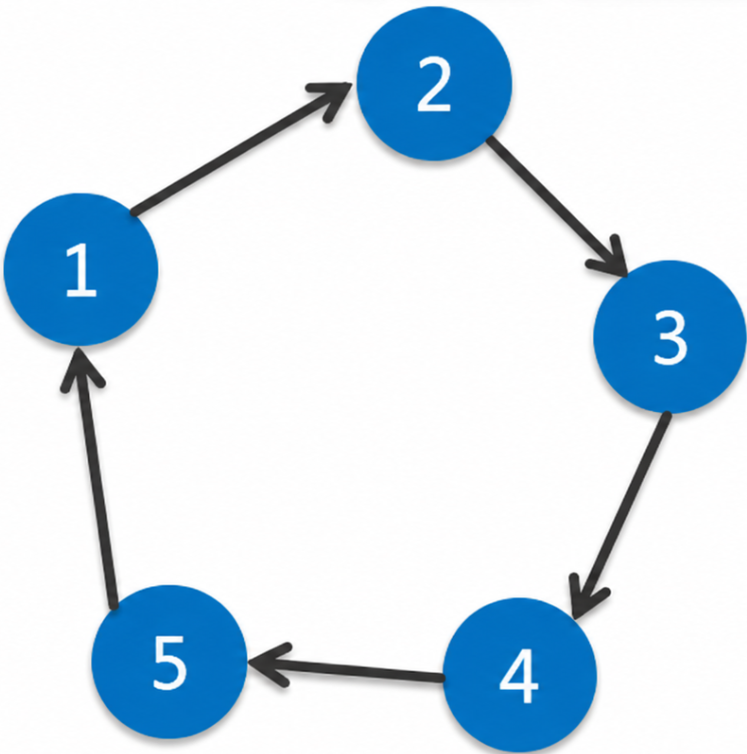
\includegraphics[width=0.2\linewidth]{images/img_20261106_171124.png}
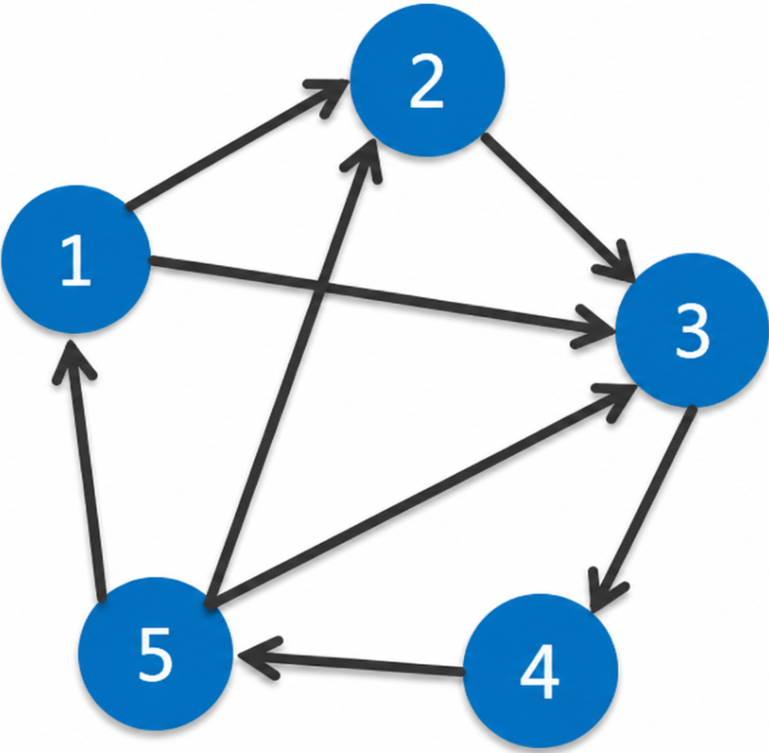
\includegraphics[width=0.2\linewidth]{images/img_20261106_171156.png}
\end{center}

\begin{itemize}
    \item \textbf{Left}: the cycle $1 \to 2 \to 3 \to 4 \to 5 \to 1$. The entire $\mathcal{S}$ is one closed irreducible finite class $\Rightarrow$ positive-recurrent; every return takes a multiple of $5$ steps $\Rightarrow$ \textbf{periodic with period $5$}.
    \item \textbf{Right}: the same cycle with extra arrows ($1 \to 3$, $5 \to 2$, $5 \to 3$, \dots). Still irreducible and finite $\Rightarrow$ positive-recurrent; but now there are cycles of different lengths whose lengths have $\gcd 1$ (e.g.\ $1 \to 3 \to 4 \to 5 \to 1$ of length $4$ and the original cycle of length $5$) $\Rightarrow$ \textbf{aperiodic}.
\end{itemize}

\textbf{Exercise}: what are the irreducible classes of the following chain?

\begin{center}
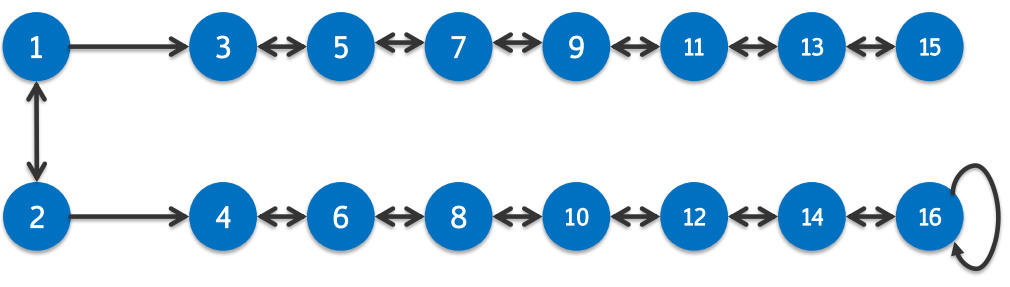
\includegraphics[width=0.707\linewidth]{images/img_20261106_171911.png}
\end{center}

\begin{itemize}
    \item $\{1, 2\}$: \textbf{transient}, \textbf{2-periodic}. It is not closed (we can leave to $3$ or $4$ and never come back); returns to $1$ only via $1 \to 2 \to 1$, i.e.\ at even times.
    \item $\{3, 5, \dots, 15\}$: \textbf{recurrent}, \textbf{2-periodic}, \textbf{absorbing}. A line with bidirectional arrows is bipartite (odd/even positions along the line), so returns take an even number of steps.
    \item $\{4, 6, \dots, 16\}$: \textbf{recurrent}, \textbf{aperiodic}, \textbf{absorbing}. Same structure, but the self-loop at $16$ breaks the periodicity.
\end{itemize}

\subsection{Examples: random walks}

\begin{itemize}
    \item \textbf{Simple random walk on $\mathbb{Z}$} (irreducible, period $2$):
    \begin{itemize}
        \item for $p = q = \frac12$ (unbiased): \textbf{null-recurrent} (even though the mode of $\mathbb{P}[X_n = i]$ is always at $0$!);
        \item for $p \neq q$: \textbf{transient} (the walk drifts to $\pm\infty$).
    \end{itemize}
    \begin{center}      
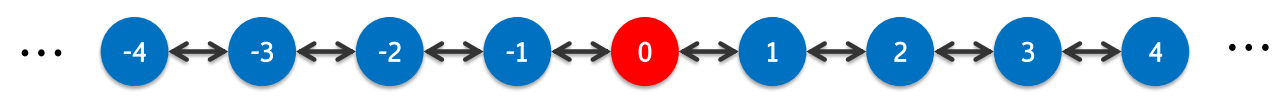
\includegraphics[width=0.707\linewidth]{images/img_20261106_172139.png}
    \end{center}
    
    \item \textbf{Simple random walk with a (reflecting) barrier at $0$} ($\mathcal{S} = \{0, 1, 2, \dots\}$):
    \begin{itemize}
        \item for $p = q = \frac12$ (unbiased): \textbf{null-recurrent};
        \item for $p > q$: \textbf{transient} (drift away from the barrier, to $+\infty$);
        \item for $p < q$: \textbf{positive-recurrent} (drift towards the barrier, the walk keeps coming back quickly).
    \end{itemize}
    \begin{center}
       
\includegraphics[width=0.707\linewidth]{images/img_20261106_172235.png}
    \end{center}
    
    \item \textbf{Unbiased random walk on $\mathbb{Z}^2$} (move to one of the $4$ neighbours uniformly): \textbf{null-recurrent}.
    \item \textbf{Unbiased random walk on $\mathbb{Z}^3$} (one of the $6$ neighbours): \textbf{transient}.
\end{itemize}

\begin{center}
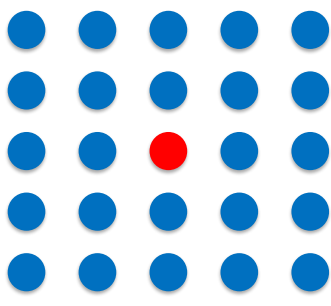
\includegraphics[width=0.2\linewidth]{images/img_20261106_172318.png} \qquad
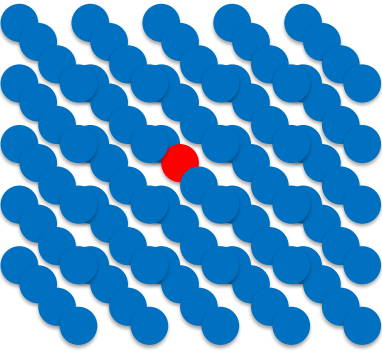
\includegraphics[width=0.2\linewidth]{images/img_20261106_172329.png}
\end{center}

\begin{remark}[Why? (not on the slides)]
Use the criterion $\sum_n p_{00}(n) = \infty \iff null$ recurrent. On $\mathbb{Z}$, returns happen only at even times and $p_{00}(2n) = \binom{2n}{n}(pq)^n$. By Stirling, $\binom{2n}{n} \sim \frac{4^n}{\sqrt{\pi n}}$, so
\[
p_{00}(2n) \sim \frac{(4pq)^n}{\sqrt{\pi n}}.
\]
\begin{itemize}
    \item If $p = q = \frac12$: $4pq = 1$ and $p_{00}(2n) \sim \frac{1}{\sqrt{\pi n}}$, whose sum diverges $\Rightarrow$ recurrent; but $p_{00}(2n) \to 0$ $\Rightarrow$ null-recurrent (by the theorem ``null $\iff p_{ii}(n) \to 0$'').
    \item If $p \neq q$: $4pq < 1$, the terms decay geometrically, the sum converges $\Rightarrow$ transient.
\end{itemize}
On $\mathbb{Z}^d$ (unbiased), $p_{00}(2n) \asymp n^{-d/2}$: the sum diverges for $d = 1, 2$ (recurrent, and null since the terms go to $0$) and converges for $d \geq 3$ (transient). A drunk man finds his way home, a drunk bird may not (Pólya).
\end{remark}

\subsection{Decomposition theorem}

\begin{theorem}[Decomposition theorem]
The state space $\mathcal{S}$ can be partitioned uniquely as
\[
\mathcal{S} = T \cup C_1 \cup C_2 \cup \cdots
\]
where $T$ is the set of \textbf{transient} states, and the $C_k$ are \textbf{irreducible closed sets of recurrent states}.
\end{theorem}

Note: we do not assert that $T$ is irreducible! $T$ may be made of several classes (or of states that do not intercommunicate at all).

\begin{proof}
Let $C_1, C_2, \dots$ be the recurrent equivalence classes of $\leftrightarrow$ (each class is either entirely recurrent or entirely transient, by the class-property theorem). They are irreducible by definition; we only need to show that they are all closed.

Suppose the contrary: there exist $i \in C_r$ and $j \notin C_r$ such that $p_{ij} > 0$. Then $j \not\to i$ (otherwise $i$ and $j$ would intercommunicate and would be in the same class). So once the chain jumps from $i$ to $j$, it can never come back to $i$:
\[
\mathbb{P}\big[X_n \neq i \text{ for all } n \geq 1 \mid X_0 = i\big] \geq \mathbb{P}\big[X_1 = j \mid X_0 = i\big] = p_{ij} > 0,
\]
which contradicts the assumption that $i$ is recurrent.
\end{proof}

So there are two possibilities for the trajectory of the chain:
\begin{itemize}
    \item either the chain stays in $T$ forever,
    \item or it is (eventually, or from the beginning) in one of the $C_r$, and stays there forever.
\end{itemize}
For finite $\mathcal{S}$, only the second scenario is possible (a finite set of transient states, each visited finitely often, cannot hold the chain forever).

\subsection{Decomposition for finite $\mathcal{S}$}

If $\mathcal{S}$ is finite:
\begin{itemize}
    \item there are \textbf{no null-recurrent states} (null recurrence only happens in infinite state spaces);
    \item \textbf{at least one} state is positive-recurrent;
    \item a class of states is positive-recurrent $\iff$ the class is absorbing (closed);
    \item a class of states is transient $\iff$ the class is non-absorbing;
    \item there exists at least one class of absorbing states;
    \item if the whole chain is irreducible, it is positive-recurrent.
\end{itemize}

\section{Limit behaviour}

\subsection{Ergodic theorem}

Periodicity is problematic for convergence. Example: $\mathcal{S} = \{1, 2\}$ with $p_{12} = p_{21} = 1$. Then
\[
p_{11}(n) = p_{22}(n) = \begin{cases} 0 & n \text{ odd}, \\ 1 & n \text{ even}, \end{cases}
\]
which does not converge!

\begin{theorem}[Ergodic theorem]
For an \textbf{irreducible aperiodic} chain (not necessarily finite),
\[
p_{ij}(n) \xrightarrow[n\to\infty]{} \frac{1}{\mu_j} =: \pi_j \qquad \text{for all } i \text{ and } j,
\]
where $\mu_j$ is the mean recurrence time of $j$ (with $1/\infty = 0$).
\end{theorem}

\textbf{Interpretation}: the long-term probability $\pi_j = p_{ij}(\infty)$ of being in state $j$ ``from anywhere'' (it does not depend on $i$: the chain forgets where it started) converges to the \textbf{rate of revisiting that state}. If, on average, we come back to $j$ every $\mu_j$ steps, then in the long run we spend a fraction $1/\mu_j$ of the time in $j$.
\begin{itemize}
    \item If the chain is positive-recurrent (ergodic), $\pi_j > 0$ for all $j$, and $\pi$ is a probability distribution.
    \item If the chain is null-recurrent or transient, $\mu_j = \infty$ and $p_{ij}(n) \to 0$ for all $i, j$: the probability mass ``escapes to infinity'' (only possible in infinite state spaces).
\end{itemize}

Can we compute that rate? Yes!

\subsection{Stationary distribution $\pi$}

\begin{definition}[Stationary distribution]
A distribution $\pi$ (row vector, $\pi_j \geq 0$, $\sum_j \pi_j = 1$) is \textbf{stationary} if
\[
\pi = \pi P.
\]
If $\boldsymbol{\mu}(0) = \pi$, then $\boldsymbol{\mu}(n) = \pi P^n = \pi$ for all $n$: the distribution of $X_n$ no longer changes.
\end{definition}

The limit of the ergodic theorem is stationary: letting $n \to \infty$ in $P^{n+1} = P^n P$, every row $\pi$ of $P^\infty$ satisfies $\pi = \pi P$.

\begin{theorem}[Spectral view, finite chains]
For an irreducible aperiodic finite Markov chain, the transition matrix $P \in \R^{d\times d}$:
\begin{itemize}
    \item has a single dominant eigenvalue $\lambda_1 = 1$; its associated (left) eigenvector is (proportional to) the stationary distribution $\pi$;
    \item all other eigenvalues satisfy $|\lambda_2|, |\lambda_3|, \dots, |\lambda_d| < 1$.
\end{itemize}
\end{theorem}

Note that $1$ is always an eigenvalue of a stochastic matrix: $P\mathbf{1}^\top = \mathbf{1}^\top$ (rows sum to one), so it is a right eigenvector; $\pi$ is the corresponding \textbf{left} eigenvector. The other eigenvalues having modulus $< 1$ is what makes $P^n$ converge (the components along them decay like $|\lambda_k|^n$; the speed of convergence is governed by $|\lambda_2|$).

\textbf{Computing the unique stationary distribution}:
\begin{itemize}
    \item solve the linear system $\pi = \pi P$ together with $\pi\mathbf{1}^\top = 1$ (normalisation; the system $\pi = \pi P$ alone only determines $\pi$ up to a constant);
    \item for large systems, use the \textbf{power method}: take a vector $e = [1, 1, \dots, 1]/d$ (for example), and repeatedly multiply by $P$: $eP^n \to \pi$. This is exactly simulating the evolution of $\boldsymbol{\mu}(n)$ from $\boldsymbol{\mu}(0) = e$.
\end{itemize}

\begin{remark}[Back to the two-state example]
Recall $P = \begin{pmatrix} 1/2 & 1/2 \\ 3/4 & 1/4 \end{pmatrix}$ and $P^{10} \approx \begin{pmatrix} 0.600 & 0.400 \\ 0.600 & 0.400 \end{pmatrix}$. Solving $\pi = \pi P$: $\pi_1 = \frac12\pi_1 + \frac34\pi_2 \Rightarrow \pi_1 = \frac32\pi_2$, and with $\pi_1 + \pi_2 = 1$:
\[
\pi = \big[3/5,\ 2/5\big],
\]
which matches the rows of $P^{10}$. The eigenvalues of $P$ are $1$ and $\operatorname{tr}(P) - 1 = -\frac14$, so $P^n$ converges to its limit like $(1/4)^n$: very fast. Consistently with the ergodic theorem, the mean recurrence times are $\mu_1 = 5/3$ and $\mu_2 = 5/2$.
\end{remark}

\section{Random walks on general graphs}

\subsection{Random walk as a Markov chain}

\begin{definition}[Random walk on a graph]
Let $G(V, E)$ be an undirected graph, assumed connected (otherwise, take $G$ to be the giant component of the actual network). The \textbf{random walk} on $G$ is the Markov chain with state space $\mathcal{S} = V$:
\begin{itemize}
    \item $X_n \in V$ is the node at time $n$;
    \item at each time step, go to a neighbour of $X_n$ chosen uniformly at random $\to X_{n+1}$.
\end{itemize}
It is a random memoryless exploration of the graph. With $d_i$ the degree of node $i$, the transition matrix is
\[
p_{ij} = \begin{cases} 1/d_i & (i, j) \in E, \\ 0 & \text{otherwise.} \end{cases}
\]
\end{definition}

\begin{center}
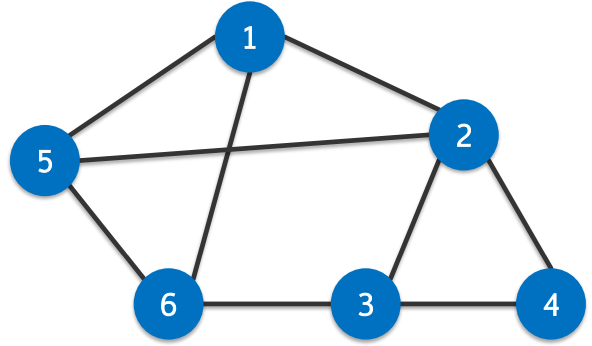
\includegraphics[width=0.4\linewidth]{images/img_20261106_183848.png}
\end{center}

If $G(V, E)$ is \textbf{undirected, connected and non-bipartite}, then $\{X_n\}$ is an \textbf{ergodic} (irreducible, aperiodic) Markov chain:
\begin{itemize}
    \item connected $\Rightarrow$ irreducible (every node can reach every other node);
    \item non-bipartite $\Rightarrow$ aperiodic: on an undirected graph, $i \to j \to i$ gives returns of length $2$; a bipartite graph has only even cycles (period $2$), whereas a non-bipartite graph has an odd cycle, giving an odd return length and hence $\gcd = 1$;
    \item finite and irreducible $\Rightarrow$ positive-recurrent.
\end{itemize}
Ergodicity then gives a stationary distribution $\pi$ with
\[
p_{ij}(n) = \mathbb{P}(\text{at vertex } j \text{ after } n \text{ steps} \mid \text{starting at vertex } i) \xrightarrow[n\to\infty]{} \pi_j \qquad \text{for all } i, j \in V:
\]
the random walk ``forgets'' its starting point $i$.

\subsection{Stationary distribution of a random walk}

\begin{theorem}[Lemma]
For the random walk on an undirected connected graph,
\[
\pi \propto [d_1, d_2, \dots, d_n], \qquad \text{i.e.} \qquad \pi_j = \frac{d_j}{\sum_i d_i} = \frac{d_j}{2|E|}.
\]
\end{theorem}

\begin{proof}
By definition, $\pi$ is stationary iff $\pi = \pi P$. Let $x = [d_1, d_2, \dots, d_n]\,P$. Then
\[
x_j = \sum_i d_i\, p_{ij} = \sum_i d_i \cdot \frac{1}{d_i}\mathbf{1}\{(i,j) \in E\} = \sum_i \mathbf{1}\{(i, j) \in E\} = d_j.
\]
So $[d_1, \dots, d_n]$ is a left eigenvector of $P$ with eigenvalue $1$, hence $\pi \propto [d_1, \dots, d_n]$ (by uniqueness of the stationary distribution of an ergodic chain); normalising uses $\sum_i d_i = 2|E|$.
\end{proof}

\textbf{Intuition}:
\begin{itemize}
    \item in the stationary regime, the random walk ``sees'' uniformly random edges (each of the $2|E|$ directed edges is traversed with the same frequency);
    \item the nodes visited by the random walk are therefore biased by their number of edges, i.e.\ their degree: high-degree nodes are visited more often.
\end{itemize}

\begin{remark}
This compact characterisation is specific to \textbf{undirected} graphs: no such simple formula for $\pi$ exists for directed graphs (in general, $\pi$ must be computed numerically, e.g.\ with the power method). Sampling nodes through a random walk is a common way to explore large networks, but it gives a degree-biased sample.
\end{remark}
